% vim: ai sw=2 spell spelllang=en

\documentclass[handout,xcolor=dvipsnames]{beamer}

\let\Oldemph\emph
\renewcommand{\emph}[1]{\textcolor{blue}{\Oldemph{#1}}}
\newcommand{\heading}[1]{\textbf{\textcolor{BurntOrange}{#1}}}

% Copyright 2004 by Till Tantau <tantau@users.sourceforge.net>.
%
% In principle, this file can be redistributed and/or modified under
% the terms of the GNU Public License, version 2.
%
% However, this file is supposed to be a template to be modified
% for your own needs. For this reason, if you use this file as a
% template and not specifically distribute it as part of a another
% package/program, I grant the extra permission to freely copy and
% modify this file as you see fit and even to delete this copyright
% notice. 


\mode<presentation>
{
%  \usetheme{Warsaw}
\usetheme{Madrid}

  \setbeamercovered{transparent}
}

\usepackage[utf8]{inputenc}
\usepackage{times}
\usepackage[T1]{fontenc}

\usepackage{graphicx}
\usepackage[final]{listings}
\usepackage{multirow}

\lstset{tabsize=2,numbers=none,showstringspaces=false,breaklines=true,
	breakatwhitespace=true,escapeinside={(*@}{@*)},
	basicstyle=\scriptsize,keywordstyle=\bfseries\color{OliveGreen},
	commentstyle=\color{blue}}

\title{Stanse}

\subtitle{Nástroj pro statickou analýzu}
% {Include Only If Paper Has a Subtitle}

\author[J. Obdržálek, J. Slabý, M. Trtík]{Jan~Obdržálek, \emph{Jiří~Slabý}, Marek~Trtík}

\institute{ITI}

\date{1. 4. 2011, Brno}

\subject{Theoretical Computer Science}
% This is only inserted into the PDF information catalog. Can be left
% out. 



% If you have a file called "university-logo-filename.xxx", where xxx
% is a graphic format that can be processed by latex or pdflatex,
% resp., then you can add a logo as follows:

% \pgfdeclareimage[height=0.5cm]{university-logo}{university-logo-filename}
% \logo{\pgfuseimage{university-logo}}



% Delete this, if you do not want the table of contents to pop up at
% the beginning of each subsection:
% \AtBeginSubsection[]
% {
%   \begin{frame}<beamer>
%     \frametitle{Outline}
%     \tableofcontents[currentsection,currentsubsection]
%   \end{frame}
% }


% If you wish to uncover everything in a step-wise fashion, uncomment
% the following command: 

%\beamerdefaultoverlayspecification{<+->}

\begin{document}

\begin{frame}
  \titlepage
\end{frame}

%%%%%%%%%%%%%%%%%%%%%%%

\begin{frame}
  \frametitle{Struktura prezentace}
  \begin{itemize}
  \item Co to \textsc{Stanse} je
  \pause
  \item Minulost
  \begin{itemize}
  \item Stav před kompletním přepisem
  \end{itemize}
  \pause
  \item Současnost
  \begin{itemize}
  \item Co nástroj umí
  \item Jaké techniky/algoritmy implementuje
  \end{itemize}
  \pause
  \item Budoucnost
  \pause
  \item Demo
  \end{itemize}
\end{frame}

\begin{frame}
  \frametitle{Co to \textsc{Stanse} je}
  \begin{itemize}
  \item Především vývojové prostředí pro návrh nových technik
  \begin{itemize}
  \item Žádná práce navíc -- vše potřebné k dispozici
  \end{itemize}
  \pause
  \item Poskytuje ale i techniky pro kontrolu kódu
  \begin{itemize}
  \item Statická analýza
  \item Jazyk C, rozšiřitelný na C\#/C++/Javu
  \end{itemize}
  \pause
  \item Vyvíjen na ITI FI
  \pause
  \item Psaný v Javě
  \begin{itemize}
  \item Kvůli jednoduchosti implementace nových technik
  \item Na druhou stranu některé nevýhody (viz dále)
  \end{itemize}
  \end{itemize}
\end{frame}

\begin{frame}
  \frametitle{Minulost}
  \heading{Formal verification, analysis, and testing of software
      systems}
  \begin{itemize}
  \item Projekt mezi ITI/ANF Data od roku 2006
  \item \emph{Cíl:} automaticky nacházet chyby a úzká místa v kódu
  \item Zaměřeno na realný kód (obsáhlé zdrojové kódy apod.)
  \end{itemize}

  \pause
  \medskip

  \heading{Stanse}
  \begin{itemize}
  \item První fungující verze v létě 2007
  \item Vyzkoušeno v ANF Data, nalezeno několik chyb
  \item Následuje kompletní přepsání
  \item V září 2009 veřejně uvolněno pod GPLv2
  \item \url{http://stanse.fi.muni.cz/}
  \end{itemize}

\end{frame}

\begin{frame}
  \frametitle{Současnost}

  \heading{Stav}
  \begin{itemize}
  \item \emph{Plná podpora ANSI C99}, včetně většiny GNU C rozšíření
    \begin{itemize}
    \item Tzn. je schopno pracovat mj. s Linuxovým jádrem
    \end{itemize}
  \item Modulární, lehce rozšiřitelný
  \item Jednoduše použitelné \emph{grafické rozhraní} a inspekce chyb
  \item Na checkerech nezávislý systém pro reportování chyb
  \item Intra- a inter-procedurální analýza
  \item Dávkové spouštění + podpora překladových systémů (\textsc{make})
  \item Webový výstup chyb
  \end{itemize}
\end{frame}


\begin{frame}
  \frametitle{Uvnitř \textsc{Stanse}}

  \heading{C parser}
  \begin{itemize}
  \item Preprocessor
  \item Strojově generovaný (\textsc{antlr})
  \begin{itemize}
  \item Relativně pomalý
  \end{itemize}
  \item Výstupem je AST v XML, CFG a graf volání
  \end{itemize}

  \pause
  \medskip

  \heading{Správa interních struktur}
  \begin{itemize}
  \item Líný přístup k parsování souborů
  \begin{itemize}
  \item Podpora rozsáhlých kódů
  \end{itemize}
  \item Knihovny pro průchod výstupu parseru
  \end{itemize}

\end{frame}

\begin{frame}[fragile]
  \frametitle{Příklad interní struktury}
  \begin{center}
  \begin{tabular}{|c|} \hline
  Zdroj \\ \hline \hline
  \begin{lstlisting}[language=C]
if (cond)
  yes();
else
  no();
  \end{lstlisting} \\
  $\Downarrow$
  \end{tabular} \\
  \begin{tabular}{|c|c|} \hline
  AST (\texttt{$--$dump$-$xml}) & CFG (\texttt{$--$dump$-$cfg}) \\ \hline\hline
  \begin{lstlisting}[language=XML]
<ifElseStatement>
  <id>cond</id>         # cond
  <expressionStatement> # true
    <functionCall>
      <id>yes</id>
    </functionCall>
  </expressionStatement>
  <expressionStatement> # false
    <functionCall>
      <id>no</id>
    </functionCall>
  </expressionStatement>
</ifElseStatement>
  \end{lstlisting}
  & \parbox[c]{2.6cm}{\includegraphics[width=2.6cm]{cond}} \\ \hline
  \end{tabular}
  \end{center}

\end{frame}

\begin{frame}
  \frametitle{Checkery}
  \heading{Vstup: výstup z parseru} \\
  \heading{Výstup: chyby předané správě chyb}

  \pause
  \medskip

  \begin{itemize}
  \item AutomatonChecker
  \item ThreadChecker
  \item LockChecker
  \item ReachabilityChecker
  \end{itemize}

\end{frame}

\begin{frame}
  \frametitle{AutomatonChecker}

  \begin{itemize}
  \item Technika jako v \textsc{xgcc} -- minulá přednáška
  \item Používá konečné automaty k popisu chybového chování
  \end{itemize}
  \begin{center}
    \input{locking.pspdftex}
  \end{center}

  \pause

  \begin{itemize}
  \item Hlídá zámky, paměť, referenční počty a podobné chyby
  \begin{itemize}
    \item Cokoli může být popsáno KA, může být i zkontrolováno
    \item Např. chybné zamykání, vnoření zámky, AB-BA deadlocky,
      dereference NULL, spaní uvnitř kritických sekcí, úniky zdrojů atd.
  \end{itemize}
  \item Vysoce flexibilní díky XML konfiguraci
  \begin{itemize}
    \item Základní konfigurace pro uživatelský prostor jsou součástí
    \item Také pro jádro (liší se ve jménech funkcí)
  \end{itemize}
  \end{itemize}
\end{frame}
  
\begin{frame}
  \frametitle{ThreadChecker}
  \begin{itemize}
  \item Hledá a sleduje chování vlákna
  \item Pozoruje zamykání a odemykání zámků (interprocedurálně)
  \item Tvoří tzv. Resource Allocation grafy
    \begin{itemize}
    \item K výpočtu závislostí zámků
    \end{itemize}
  \item Proloží vytvořené grafy všech vláken a hledá cykly
  \item Nachází netriviální problémy se zámky mezi vlákny
  \end{itemize}

  \begin{center}
    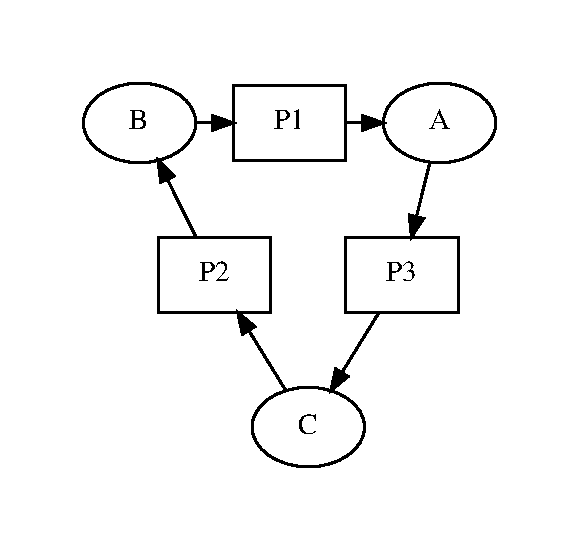
\includegraphics[width=5cm]{RAG}
  \end{center}
\end{frame}
  
\begin{frame}
  \frametitle{LockChecker}

  \begin{itemize}
  \item Statistická analýza
  \end{itemize}

\end{frame}
  
\begin{frame}
  \frametitle{ReachabilityChecker}
  \begin{itemize}
  \item Reports unreachable (dead) code.
  \item Only 200 lines long.
  \item It serves only as a framework demonstration.
    \begin{itemize}
    \item But found few bugs as well: \texttt{\textbf{if} (error)\underline{;}
      \textbf{return};}
    \end{itemize}
  \end{itemize}

\end{frame}

\begin{frame}[fragile]
  \frametitle{Configuration}
  \heading{Automaton Checker configuration example}
  \begin{lstlisting}[language=XML]
<automaton>
  <start state="U" />

  <transition from="U[A]" by="lock[A]" to="L[A]" />
  <transition from="L[A]" by="unlock[A]" to="U[A]" />

  <error from="U[A]" by="unlock[A]" desc="double unlock" ... />
  <error from="L[A]" by="lock[A]" desc="double lock" ... />

  <pattern name="lock">
    <functionCall>
      <id>__st_mutex_lock_st__</id>
      <var name="A" />
    </functionCall>
  </pattern>
  <pattern name="unlock">
    <functionCall>
      <id>__st_mutex_unlock_st__</id>
      <var name="A" />
    </functionCall>
  </pattern>
</automaton>
  \end{lstlisting}
\end{frame}

\begin{frame}[fragile]
  \frametitle{Worked Example}
  Having the configuration above and a project:
  \begin{center}
  \begin{tabular}{|l|l|} \hline
  Source (\texttt{my.c}) & \texttt{Makefile} \\ \hline \hline
  \begin{lstlisting}[language=C]
1 void bad_locking(struct mutex *my_lock,
2                  int cond)
3 {
4   mutex_lock(my_lock);
5   if (cond)
6     mutex_lock(my_lock);
7 }
  \end{lstlisting}
  &
  \begin{lstlisting}[language=make]
CFLAGS=-Wall -O2
CC=gcc

all: my.o
  \end{lstlisting} \\ \hline
  \end{tabular}
  \end{center}

  \pause

  \textsc{Stanse} can find bugs: \\
{\scriptsize\texttt{%
\textcolor{red}{\$ stanse -c AutomatonChecker:conf.xml $--$makefile
'Makefile'} \\
\pause
Error(s) found: \\
my.o.preproc, line 6: $\{$AutomatonChecker of conf.xml$\}$ in function 'bad\_locking' double lock [traces: 1] \\
trace [locations: 4] \\
start[file: my.o.preproc, line: 4] \\
middle[file: my.o.preproc, line: 5] \\
middle[file: my.o.preproc, line: 5] \\
end[my\_lock][file: my.o.preproc, line: 6] \\
}}

\end{frame}

\begin{frame}
\frametitle{Tools Comparison}
\heading{There are many tools available, some of them are compared here}
\begin{tabular}{l|ccccl}
\multirow{2}{*}{Tool name} &
Open- &
Confi- &
Batch &
Inter- &
\multirow{2}{*}{Languages} \\
%Tool name        & Open & Confi-  & Batch   & Inter- & Languages
                  & source & gurable & support & proc.  & \\ \hline
\textsc{Coverity} & no   & yes     & yes     & yes    & GC, C++, C\#, Java \\
\textsc{Klocwork} & no   & yes     & yes     & yes    & GC, C++, C\#, Java \\
\textsc{Splint}   & yes  & no      & no      & no     & C \\
\textsc{Sparse}   & yes  & no      & yes     & no     & GC \\
\textsc{Clang}    & yes  & no      & no      & no     & GC$^*$, C++, Obj-C \\
\textsc{Uno}      & yes  & yes     & no      & yes    & C$^\dagger$ \\
\textsc{Stanse}   & yes  & yes     & yes     & yes    & GC \\
\textsc{FindBugs} & yes  & no      & yes     & no     & Java \\ \hline
\multicolumn{6}{l}{\footnotesize GC stands for GNU C.} \\
\multicolumn{6}{l}{\footnotesize $^*$\textsc{Clang} is still under heavy
development, its GNU C support is incomplete.} \\
\multicolumn{6}{l}{\footnotesize $^\dagger$C support in \textsc{Uno} does not
even implement full C99.} \\
\end{tabular}
\end{frame}

\begin{frame}
  \frametitle{Found Bugs I.}
  
  \heading{ANF Data}
  \begin{itemize}
  \item \texttt{malloc()} not tested against NULL.
  \item Memory leaks.
  \end{itemize}

  \pause
  \medskip

  \heading{Linux kernel}\\
  Over 70 of the following kind of errors (reported and fixed):
  \begin{itemize}
  \item Pointer usage violations
  \item Locking discipline errors
    \begin{itemize}
    \item I.e. potential real-world deadlocks (an example follows).
    \end{itemize}
  \item Function pairing
    \begin{itemize}
    \item E.g. get\_cpu/put\_cpu, interrupt disable/enable, etc.
    \end{itemize}
  \item Unreachable code
  \end{itemize}

  \pause
  \medskip

  \heading{Other code}
  \begin{itemize}
  \item CESNET (Czech backbone) project developing HW accelerators.
  \item Small libraries/tools (acl, attr).
  \end{itemize}
\end{frame}

\begin{frame}[fragile]
  \frametitle{Found Bugs II.}

  \heading{One simple kernel example}

  Source: \texttt{\small linux-2.6.28/drivers/pci/hotplug/pciehp\_core.c}
  \begin{lstlisting}[language=C]
static int set_lock_status(struct hotplug_slot *hotplug_slot,
                           u8 status)
{
  struct slot *slot = hotplug_slot->private;
  ...
  mutex_lock(&slot->ctrl->crit_sect);

  /* has it been >1 sec since our last toggle? */
  if ((get_seconds() - slot->last_emi_toggle) < 1)
    return -EINVAL;
  ...
  mutex_unlock(&slot->ctrl->crit_sect);
  return 0;
}
  \end{lstlisting}

  Trigger: \texttt{\small echo '1' > /sys/bus/pci/slots/.../lock} twice in 1s

  \pause
  \medskip
  Full list at \url{http://stanse.fi.muni.cz/bugs.html}.

\end{frame}

\begin{frame}[fragile]
  \frametitle{False Positives}
  Oscillating between 30 and 70\% -- depending on checker and source codes,
  but indeed quite high.

  \medskip
  \pause

  \heading {Fighting FP}
  \begin{itemize}
  \item Improving configuration.
  \begin{itemize}
    \item The quality is important and alters directly the FP-to-bugs ratio.
      \begin{itemize}
      \item Too naive automata results in high FP ratio.
      \end{itemize}
    \item Prune bugs in the configuration proper.
    \item Tune-up based on previous results.
  \end{itemize}
\pause
  \item FP detectors: a Java code finding certain patterns.
  \begin{itemize}
    \item E.g. leaks of memory pointer by globals are mostly a FP.
  \end{itemize}
\pause
  \item Better or new analyses/checkers.
  \begin{itemize}
    \item Inappropriate (non-sophisticated) techniques.
      \begin{itemize}
      \item E.g. no bugs of such type present in the code.
      \end{itemize}
    \item Symbolic execution or simple simulation to ensure the
      paths are reachable.
  \end{itemize}
  \end{itemize}

\end{frame}

\begin{frame}
  \frametitle{Work in Progress}
  \heading{Points-to analysis (Master's thesis)}
  \begin{itemize}
  \item Improves knowledge about values in pointers for more exact analyses.
  \item Memory checker knows which pointers point to the same objects.
  \end{itemize}

  \pause
  \medskip

  \heading{Statistical approach (Master's thesis)}
  \begin{itemize}
  \item Intended for the locking checker.
  \item Tracks which variables are altered under which locks.
  \item Based on a technique used in \textsc{Metal}.
  \end{itemize}

  \pause
  \medskip

  \heading{Plugin for IDE (Bachelor's thesis)}
  \begin{itemize}
  \item Plugin for Eclipse, Netbeans.
  \item For easier deployment of the tool (immediate response).
  \end{itemize}

  \pause
  \medskip

  \heading{Symbolic execution}
  \begin{itemize}
  \item Part of Marek's and my dissertation.
  \item Needn't be part of \textsc{Stanse}.
  \end{itemize}
\end{frame}


\begin{frame}
  \frametitle{Future Work}
  \heading{Get rid of XML}
  \begin{itemize}
  \item XML is a beast in memory consumption.
  \item Switch to standard Java objects.
    \begin{itemize}
    \item The ones returned from parser? Language dependency!
    \end{itemize}
  \end{itemize}

  \pause
  \medskip

  \heading{Java to C switch}
  \begin{itemize}
  \item Generated parser is slow.
    \begin{itemize}
    \item It is yet to be optimized by \texttt{antlr3} authors.
    \end{itemize}
  \item Method invocation is not the fastest operation in Java.
  \end{itemize}

  \pause
  \medskip

  \heading{Better preprocessor}
  \begin{itemize}
  \item Currently we have none.
  \item Nothing binds preprocessed line numbers to original ones.
  \end{itemize}

\end{frame}

\begin{frame}
  \frametitle{Conclusion}
  \begin{itemize}
  \item \textsc{Stanse} is still in the \emph{early phase} (read: still much
    work to do).
    \begin{itemize}
    \item There is a work in progress.
    \end{itemize}
  \item It is not only a checker, it is rather a \emph{platform/framework}.
  \item However it \emph{found many bugs} in real-world large code base.
  \item Visit \url{http://stanse.fi.muni.cz/} for more info.
  \end{itemize}

  \pause
  \vfill
  \begin{center}
    \emph{We want to hear about your problems! *}
  \end{center}

  \vfill
  {\tiny * Applies only to problems related to bugfinding.}
\end{frame}

\begin{frame}
  \frametitle{Discussion}
  \begin{center} \huge
  Thank you for your attention! \\[2.4em]
  Questions?
  \end{center}
\end{frame}

\end{document}

